\chapter{Temperature distribution of a toy glacier}

\modinfo{Directory}{ToyGlacierTemperature}
\modinfo{Solvers}{\Idx{HeatSolver}} 
\modinfo{Tools}{\Idx{ElmerGUI},\Idx{nglib}} 
\modinfo{Dimensions}{2D, Steady-state}
\modinfo{Author}{Peter R{\aa}back, Thomas Zwinger}


\subsection*{Introduction}

The purpose of this simple tutorial is to be an introduction into Elmer for people dealing with computational glaceology.
This tutorial shows how to apply one equation and related boundary conditions to just one domain.


\subsection*{Problem description}

Consider a 2D toy model of a glacier with length of 7000~m and thickness of about 1000~m. 
There is a slight declination in the geometry which will make the glacier flow to the left. 
The left-hand-side is rounded to imitate a true glacier while the right-hand-side is 
cut off. 

\begin{figure}
\begin{center}
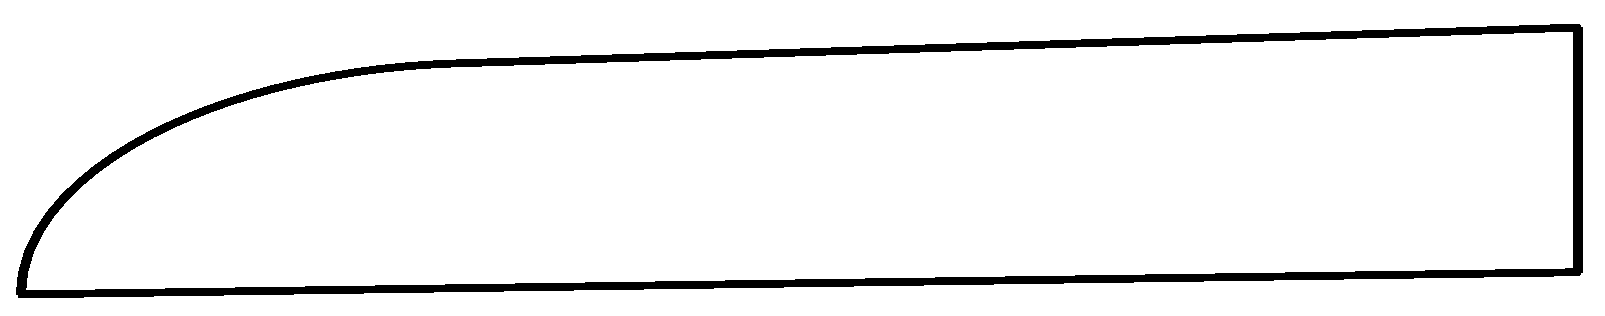
\includegraphics[width=120mm]{glacier_toy_shape}
\caption{The shape of the toy glacier to be studied}\label{glac:shape}
\end{center}
\end{figure}

We solve for the temperature distribution $T$ of the glacier. 
A heat flux of $q=0.02$~W/m$^2$ is applied at the bottom of the glacier while the surface stays at a
fixed temperature of $T_0=-10$~C. The material properties of ice are used for the 
heat conductivity $\kappa(T)$. 
The temperature distribution in the glacier 
may be solved from
\begin{equation}
\left \{
\begin{array}{cccc}
- \kappa \Delta T &= & 0 & \mathrm{ in } \, \, \Omega \\
T&=&T_0 & \mathrm{ on } \, \, \Gamma_D \\
\kappa \frac{\partial T}{\partial n} &=& q & \mathrm{ on } \,\, \Gamma_N \\
\end{array}
\right .
\end{equation}

\subsection*{Starting and meshing}

Start \texttt{ElmerGUI} from command line or by clicking the icon in your desktop (or in the /bin directory of you installation). 
Here we describe the essential steps in the ElmerGUI by writing out the clicking procedure. Tabulation generally means that the 
selections are done within the window chosen at the higher level. 

The mesh is given in ElmerGrid format in file \texttt{glacier\_toy.in2d} in the samples directory of ElmerGUI, 
load this file.
\ttbegin
File 
  Open -> glacier\_toy.in2d
\ttend
You should obtain a mesh consisting of just two triangular elements. The mesh is created by the \texttt{netgen} plugin 
and in order to increase the mesh density the in-line parameters of netgen must be defined in ElmerGUI.
Here we set the maximum element size to 50. 
\ttbegin
Mesh
  Configure... 
    nglib -> Max H: 50
\ttend
The resulting mesh should consist of 3335 nodes and 6355 triangles as may be checked in the 
\texttt{Model summary} window.
%If the mesh was successfully imported your window should look something in figure~\ref{glac:mesh}.

%\begin{figure}
%\begin{center}
%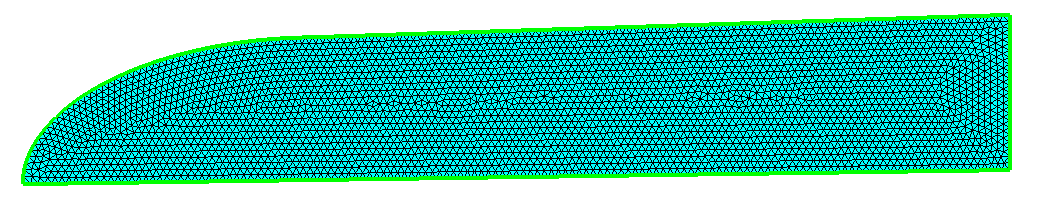
\includegraphics[width=120mm]{glacier_toy_mesh}
%\caption{The finite element mesh in ElmerGUI}\label{glac:mesh}
%\end{center}
%\end{figure}

\subsection*{Command file definition}

After we have the mesh we start to go through the Model menu from the top to bottom. 
In the \texttt{Setup} we choose things related to the whole simulation such as file names, 
time stepping, constants etc.
The simulation is carried out in 2-dimensional cartesian
coordinates and in steady-state. 
Only one steady-state iteration is needed as the case is linear. 
\ttbegin
Model
  Setup 
    Simulation Type = Steady state
    Steady state max. iter = 1
\ttend
Choose \texttt{Accept} to close the window.

In the equation section we choose the relevant equations and parameters related to their solution. 
In this case we'll have one set only one equation -- the heat equation.


When defining Equations and Materials it is possible to assign the to bodies immediately, or to use mouse
selection to assign them later. In this case we have just one body and one boundary and therefore its easier to assign 
the Equation and Material to it directly.

For the linear system solvers we are happy to use the defaults. One may however, try out different
preconditioners (ILU1,\ldots) or direct Umfpack solver, for example.
\ttbegin
Model
  Equation
    Add 
      Name = Heat Equation
      Apply to bodies = 1
      Heat Equation
        Active = on
  Apply   
  OK
\ttend        

The Material section includes all the material parameters.
They are divided to generic parameters which are direct properties of the material
without making any assumptions on the physical model, such as the mass. Other properties assume
a physical law, such heat conductivity.
We choose ice from the Material library which automatically sets for the needed material properties. 
\ttbegin
Model
  Material
    Add 
      Material library
        Water (frozen)
      Apply to bodies = Body 1 
      Add 
      OK
\ttend
This includes, for example, temperature dependent heat conductivity as may be seen under the HeatEquation page of
the material properties. MATC language is used here to define the functional form.


A Body Force represents the right-hand-side of a equation that in this case represents
the heat source. In this case there are no internal heat sources so we do not need one.
Also no Initial Condition is required in steady state case.

\begin{figure}
\begin{center}
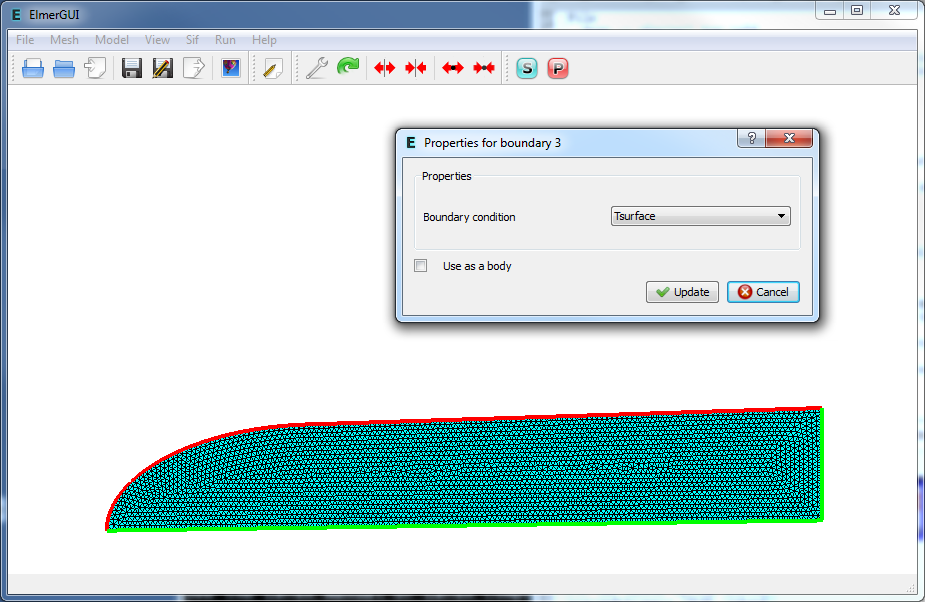
\includegraphics[width=120mm]{glacier_toy_gui}
\caption{Defining boundary conditions in ElmerGUI session}\label{glac:bc}
\end{center}
\end{figure}

We set three different kinds of boundary conditions. A fixed temperature, a fixed 
flux and natural boundary condition (zero flux). As there are several boundaries
we first define the different boundary types, and thereafter assign them using the mouse.
A screenshot of the case when setting the BCs is shown in figure~\ref{glac:bc}.

\ttbegin
Model
  BoundaryCondition
    Add 
      Heat Equation
        Temperature = -10.0
      Name = Tsurface
      OK
    Add 
      Heat Equation
        Heat Flux = 0.02
      Name = Tflux
      OK
    Add 
      Name = Tnatural
      OK
\ttend   
Then we set the boundary properties 
\ttbegin
Model 
  Set boundary properties  
\ttend
Choose the correct boundary by clicking with the mouse
and apply the condition for this boundary.
\ttbegin
Boundary condition
  Click top boundary -> choose Tsurface
  Click bottom boundary -> choose Tflux
  Click r.h.s. boundary -> choose Tnatural
\ttend

\subsection*{Saving and solution}

For the execution 
ElmerSolver needs the mesh files and the command file. We have know basically defined
all the information for ElmerGUI to write the command file. After writing it we may also visually 
inspect the command file.
\ttbegin
Sif 
  Generate
  Edit -> look how your command file came out  
\ttend

Before we can execute the solver we should save the files in a directory. In saving the project all the
necessary files for restarting the case will be saved to the 
destination directory.
\ttbegin
File 
  Save Project
\ttend

After we have successfully saved the files we may start the solver
\ttbegin
Run
  Start solver
\ttend
A convergence view automatically pops up showing relative changes of each iteration.
The heat conductivity of ice is set to be dependent on temperature and this results to a 
nonlinear iteration.
The resulting output is shown in figure~\ref{glac:conv}.

\begin{figure}
\begin{center}
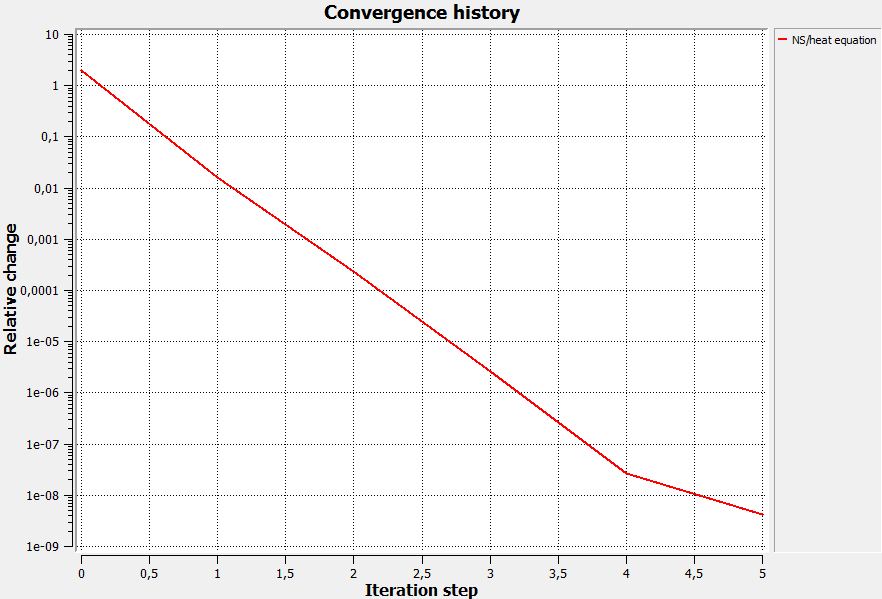
\includegraphics[width=100mm]{glacier_toy_convergence}
\caption{The convergence  ElmerGUI}\label{glac:conv}
\end{center}
\end{figure}

Note: if you face problems in the solution phase and need to edit the setting, always remember to save
the project before execution.

\subsection*{Results}

To view the results we use Paraview,
\ttbegin
Run
  Start Paraview
\ttend
Picture~\ref{glac:figtemp} shows
the surface mesh colored with temperature.
Note that these results were carried out with the obsolite
VTK based tool within ElmerGUI, and therefore look different than in Paraview.

\begin{figure}
\begin{center}
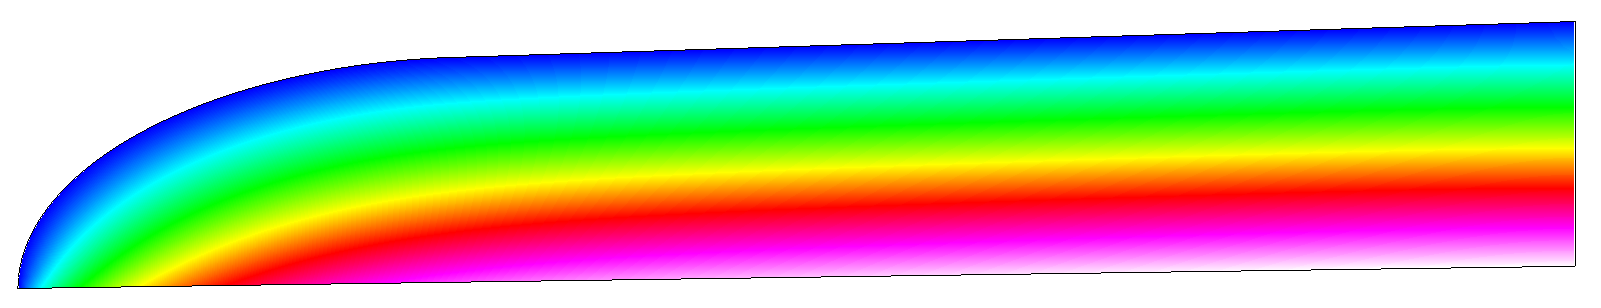
\includegraphics[width=120mm]{glacier_toy_temp}
\caption{The temperature distribution of the toy glacier.}\label{glac:figtemp}
\end{center}
\end{figure}


The maximum temperature obtained with the above choices is 0.11166~C. 
With a denser mesh the result is
naturally more accurate, but solving the problem takes more calculation time.

You may study the effect of mesh refinement by choosing 
a different value for the \texttt{Max H} parameter.
under \texttt{Configure}. After choosing \texttt{Remesh} and saving the mesh 
the solver may be recalled with the modified mesh.


\section*{Transient simulation}

We use the steady-state simulation presented above as our starting point and 
solve a transient version of it. Initially the glacier is assumed to be at -10~C 
and it is gradually heated from below. 


We use 2nd order bdf time-stepping method is selected with 100 steps
and with step size of 100 years - melting the ice from below with such a small flux 
would take quite a few years. 
The mathematical expression followed 
by ``\$'' is evaluated when the command file is read.
Here it is used to transform the time in years to those in one second. 
\ttbegin
Model
  Setup 
    Simulation Type = Transient
    Time Stepping Method = bdf
    BDF Order = 2
    Time Step Intervals = 100
    Time Step Sizes = \$ 3600 * 24 * 365.25 * 100
    Gravity = ...
\ttend

Initial conditions should be given to transient cases. In this case we choose a constant Temperature 
of -10~C. This is consistant with the boundary condition at the top wall.
\ttbegin
Model
  Initial Condition 
    Name = Initial Guess
    Heat Equation
      Temperature = -10.0
\ttend

\begin{figure}
\begin{center}
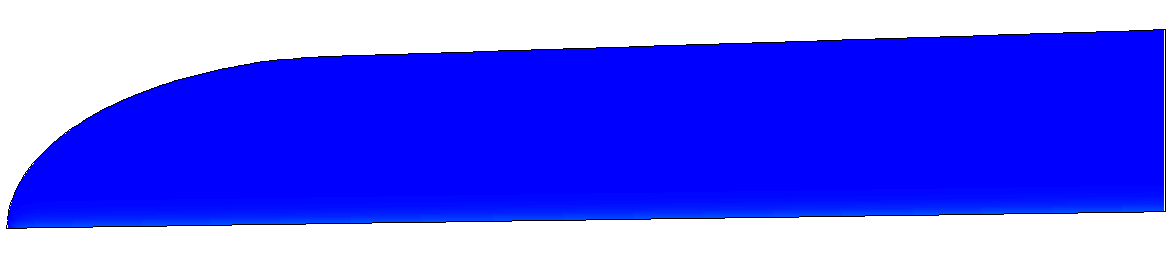
\includegraphics[width=120mm]{glacier_t1}
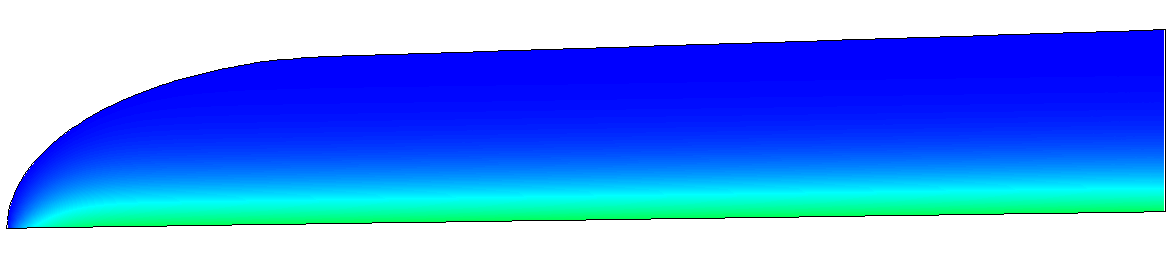
\includegraphics[width=120mm]{glacier_t20}
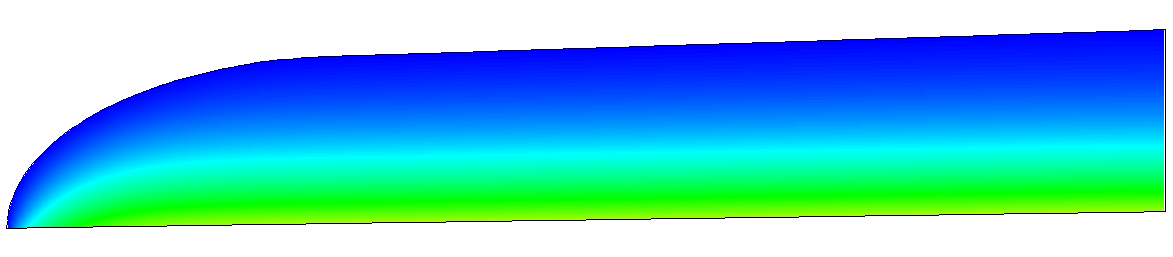
\includegraphics[width=120mm]{glacier_t50}
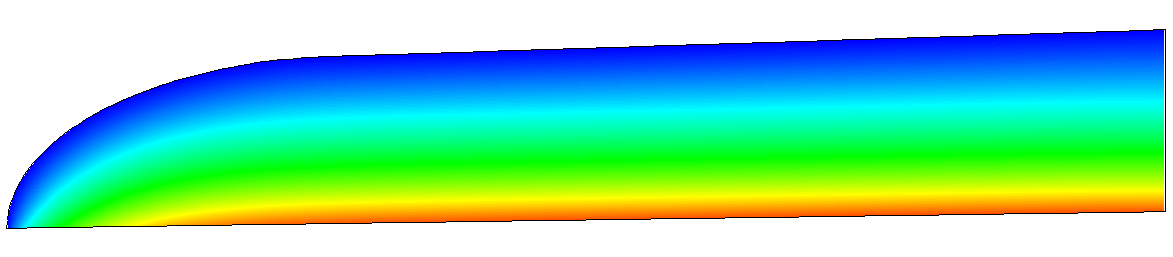
\includegraphics[width=120mm]{glacier_t100}
\caption{Temperature distribution after 1, 20, 50 and 100 timesteps. The temperature scale is the 
same that is used in the steady-state case. The maximum temperature at end should be about -3.7611~C.}
\end{center}
\end{figure}

\hfill
\mbox{}






